\chapter{Work Done}
\section{User Interface}
\subsection{Initial Assessment}
{\normalsize A basic user interface had to be developed for the website with all the functionalities that are to be provided to the user as well as the admin.
Initial assessment of the user interface proposed the following functionalities : 
\begin{itemize}
    \item Login/SignUp : for registering the user 
    \item Profile : for maintaining the profile of the user and to keep a record of the dishes prepared, robots used, recipes generated
    \item Profile : for maintaining the profile of the user and to keep a record of the dishes prepared, robots used, recipes generated
    \item Recipe Status : for giving a real time update on how the dish is being cooked and what all steps are being taken.
    \item Record : for giving step by step atomic instructions to the mechanical chef 
\end{itemize}
}
\subsection{Final Module}
{\normalsize The final UI was developed using HTML, CSS, Bootstrap and JavaScript to keep a simple user friendly design for controlling the robot using the website. \\[0.1in]
Although this final module is built using primitive tech stack, the efficiency of the design is notable as it is able to handle multiple simulator polling along with basic requests from the users.\\[0.1in]
The HTML templates form up the templates part of the MVT (Model|View|Template) architecture of the django framework. These templates are stored inside the django project folder and are rendered using the views.py file corresponding to the the requested API.
}
\section{Backend and Server}
\subsection{Initial Assessment}
{\normalsize As already mentioned, the backend was to be developed in Django for its unique and developer friendly characteristics. It is very versatile and supports rapid application development. \\[0.1in]
The initial database that looked like this : \\[0.1in]
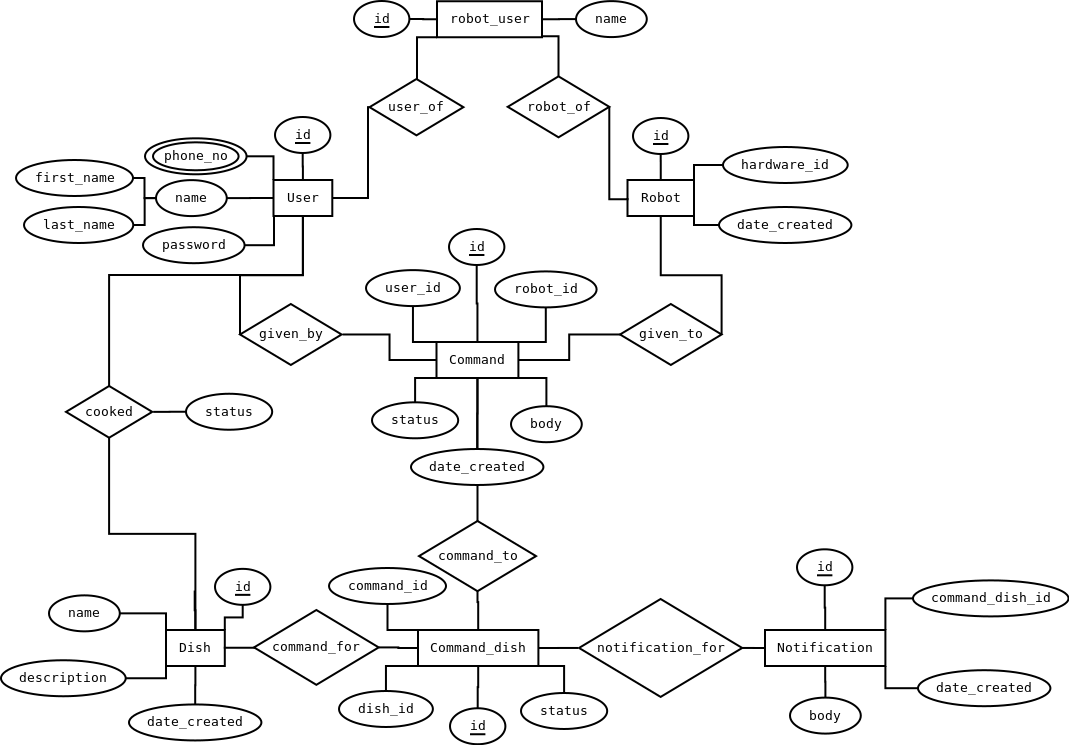
\includegraphics[width=0.8\textwidth]{mechchef.png}\\
We implemented the following changes to the database : 
\begin{itemize}
    \item Clubbing together Command, Command\_dish and Dish to make a Recipe table
    \item Dishes will be a separate table for storing the dishes that have been cooked by a person 
    \item Adding a Login/SignUp functionality
\end{itemize}
The biggest question that arose initially was to decide where to host the server? Initially the server was hosted on the machine itself but we thought of another plan to host the server. 
}
\subsection{Detailed Description}
{\normalsize We had three choices for hosting the server : 
\begin{itemize}
    \item Solution \#1 : Hosting the web server on Raspberry Pi itself that is accessible to internet.
    \item Requirements :  
    \begin{itemize}
    \renewcommand{\labelitemi}{$\Rightarrow$}
    \item Internet connection on the Raspberry Pi
    \item An operating system on the Raspberry Pi (like Raspbian)
    \item SSH access on Pi for remote access
    \item Need a domain name for linking with the Pi’s address
    \end{itemize}
    
    \item Technique : Port Forwarding to the Raspberry Pi at port not 80 \\[0.1in]
    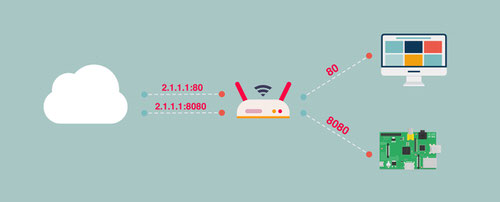
\includegraphics[width=0.8\textwidth]{2.jpg}
    \item Drawbacks
    \begin{itemize}
    \renewcommand{\labelitemi}{$\Rightarrow$}
    \item Raspberry Pi is still not as powerful as standard home PC.
    \item Crash with heavy requests.
    \item Won’t be able to access the net because of all the traffic.
    \item ISPs won’t allow hosting a commercial server.
    \end{itemize}
    
    \item Solution \#2 : Hosting a web server on Raspberry Pi itself that can be accessed by any device on the same network i.e. on localhost 

    \item Requirements :  
    \begin{itemize}
    \renewcommand{\labelitemi}{$\Rightarrow$}
    \item Install dependencies required, mentioned in the article
    \item Run Django server on local host
    \item Edit the localhost address to Raspberry Pi IP 
    \item Access Raspberry Pi through any device on the same network
    \end{itemize}
    
    \item Technique : Run the Django server locally on Pi
    \item Drawbacks
    \begin{itemize}
    \renewcommand{\labelitemi}{$\Rightarrow$}
    \item Can’t access MechChef through net but can be operated very easily using any device on local network 
    \item Will fail to achieve the required remote access
    \end{itemize}
    
    \item Solution \#3 : To communicate with server hosted online with Pi as a client 

    \item Requirements :  
    \begin{itemize}
    \renewcommand{\labelitemi}{$\Rightarrow$}
    \item Internet connection on the Raspberry Pi
    \item An operating system on the Raspberry Pi (like Raspbian)
    \item SSH access on Pi for remote access
    \item Send excel file to putty for easy access 
    \end{itemize}
    
    \item Technique : Use http protocols to access the online server and making requests (through polling)
    \item Drawbacks
    \begin{itemize}
    \renewcommand{\labelitemi}{$\Rightarrow$}
    \item Can only access mechchef through net
    \item Cannot create local network for quick use

    \end{itemize}
    
\end{itemize}
}
\subsection{Final Module}
{\normalsize The third solution was the most flexible solution and was incorporated into the final design of the server communication with the raspberry pi. This also ensured the independence of communication between server and machine without knowing the IP address of the machine or punching holes into the firewall of any wifi router. 
}
\section{APIs Built}
\subsection{Initial Assessment}
{\normalsize The API that were thought of initially were based on the database architecture that was already being used in the previous website, they lacked a lot of important details and were reformed after a brainstorming session. \\[0.1in]
}
\subsection{Final Module}
{\normalsize The final APIs planned were as follows : 
    \begin{itemize}
        \item / : GET 
        \item /about : GET
        \item /user : GET
        \item /user/{id} : GET PATCH DELETE
        \item /user/signup : POST 
        \item /user/login : POST
        \item /user/logout : POST
        \item /recipe : GET POST
        \item /recipe/{id} : GET PATCH DELETE
        \item /robot : GET 
        \item /robot/{id} : GET 
        \item /robot/vessels/{id} : GET
        \item /robotuser/{user\_id} : GET POST
        \item /robotuser/{user\_id}/{robot\_id} : GET PATCH DELETE
        \item /status/{user\_id} : GET POST
        \item /status/{user\_id}/{order\_id} : GET PATCH DELETE
        \item /status/{user\_id}/{order\_id}/{robot\_id}/loading : GET
        \item /api/robot\_id/fetch : GET
        \item api/robot\_id/user\_id/order\_id/fetch : GET
        \item /camera : GET POST
    \end{itemize}
}
\section{Polling and Simulator}
\subsection{Initial Assessment}
{\normalsize For writing the initial simulator we used a basic python code for a very shabby state based program that did not differentiate between the models used, views, controller or observer. \\[0.1in]

The initial poller was developed using the predefined python library called polling. This library supported many functions for checking the status of polling but did not provide enough means to access the information fetched after polling so we had to build our very own polling module.
}
\subsection{Detailed Description}
{\normalsize We found a couple of ways to build the simulator, one of which included using an MVC design pattern to construct the architecture of the simulator. \\[0.1in]
After reading through the "Design Patterns Elements of Reusable Object-Oriented Software" book, we managed to build the Simulator using the MVC model along with an Observer, it consisted of five modules : 
\begin{itemize}
    \item Simulator Module : For simulating the state transitions with given inputs
    \item Controller Module : For fetching information from the Views module and relaying them to the Simulator module
    \item View Module : For interacting with the user and taking inputs
    \item Observer Module : For displaying the outputs from the Controller to any platform (maybe command line or web)
    \item Poller Module : It was a customized polling module that was used to make requests to the server and update the states based on inputs given by the user
\end{itemize}
}
\subsection{Final Module}
{\normalsize The final module was built as planned as it provides a structured way to view the control flow and was easier to test. The unittest library of python was used to perform unit testing of the simulator based on multiple test cases.
}
\section{Video Streaming}
\subsection{Initial Assessment}
{\normalsize The final part of the internship was to finish the video streaming module of the simulator to fetch a video stream from the machine and show live feed on the website as the recipe is being cooked. 
}
\subsection{Detailed Description}
{\normalsize There existed three solutions for implementing the Video Streaming Module 
\begin{itemize}
    \item Solution\#1: Embedding the mjpeg video feed inside an HTML tag within the views of the website.
    \item Pros and Cons : 
    \begin{itemize}
    \renewcommand{\labelitemi}{$\Rightarrow$}
    \item It was the easiest way to video stream data from the raspicam to the website and was pretty efficient 
    \item It required the IP address of the Raspberry Pi thereby defeating the purpose of using polling altogether
    \end{itemize}
    
    \item Solution\#2: Using UV4L streaming server on raspberry pi to send video feed to the server.
    \item Pros and Cons : 
    \begin{itemize}
    \renewcommand{\labelitemi}{$\Rightarrow$}
    \item It was pretty difficult to fetch the video stream from the UV4L server and re-stream the fetched stream from raspicam on the website
    \item The functionalities provided by the UV4L server were very advanced and could be put to good use
    \end{itemize}
    
    \item Solution\#3: A very basic solution was to send snapshots from the raspicam to the website and displaying the snapshots in realtime on the website.
    \item Pros and Cons : 
    \begin{itemize}
    \renewcommand{\labelitemi}{$\Rightarrow$}
    \item It was fairly easy to implement after learning about the static and media files in django developement
    \item It did not require IP address in the Raspberry Pi
    \item It was near realtime unlike the other two solutions which were actually real time video feed
    \end{itemize}
    
\end{itemize}
}
\subsection{Final Module}
{\normalsize For implementing a cost effective and simple solution we used the third solution as it fulfilled the criteria set up through polling and could easily be integrated along with the poller module.
}
 




